\chapter{Requirement Analysis and Specification}
\label{ch:requirementanalysis}
Before designing a piece of software, it is important to have a good understanding of what the final product is supposed to do. During the requirements analysis phase, a number of steps were taken before assembling a list of requirements. First of all, a target audience questionnaire was produced and sent out to the potential application users. The results of the survey were then compiled and analysed. Secondly, a number of existing websites that could at least partly solve the problem outlined in the ”Problem Statement” \ref{sec:problemsaddressed_intro}  were examined and evaluated. Finally, a list of functional and non-functional requirements covering all the aspects of the future web application was developed and documented in this report.

\section{Target Audience Questionnaire}
\label{sec:targetaudiencequestionnaire_req}
The target audience research aims to gather information on the way football punters make their betting decisions. Questions were specifically tailored to find out what kind of content would appeal to the potential users of the application \ref{sec:targetaudience_intro}. Due to the spread of target users, an online questionnaire was used to collect the answers. There were only 9 respondents due to the specificity of the topic. A full breakdown of the questions asked and the answers received can be found in the appendices \ref{ch:questionnaire_appendix}.

\begin{figure}[H]
	\begin{center}
		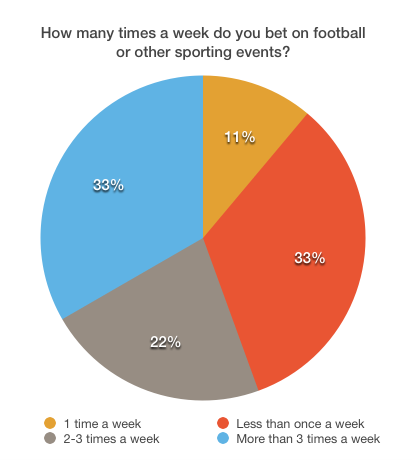
\includegraphics[width=.50\columnwidth]{req/images/howMuchDoYouBet.png}
		\caption{A pie chart illustrating the answers of the questionnaire respondents when asked how many times a week do they bet.} \label{fig:using:howmuchdoyoubet}
	\end{center}
\end{figure}

As it can be seen from figure \ref{fig:using:howmuchdoyoubet}, most of the survey participants are active punters, with the number of placed bets 2 or more per week.

\begin{figure}[H]
	\begin{center}
		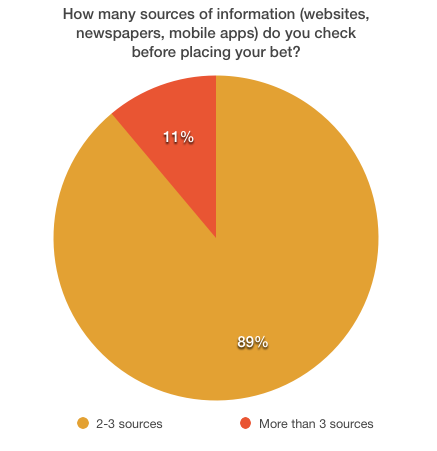
\includegraphics[width=.50\columnwidth]{req/images/howManySources.png}
		\caption{A pie chart displaying the answers of the respondents when asked how many sources of information (websites, newspapers, mobile apps) do they check before placing a bet.}
		\label{fig:using:howmanysources}
	\end{center}
\end{figure}

\begin{figure}[H]
	\begin{center}
		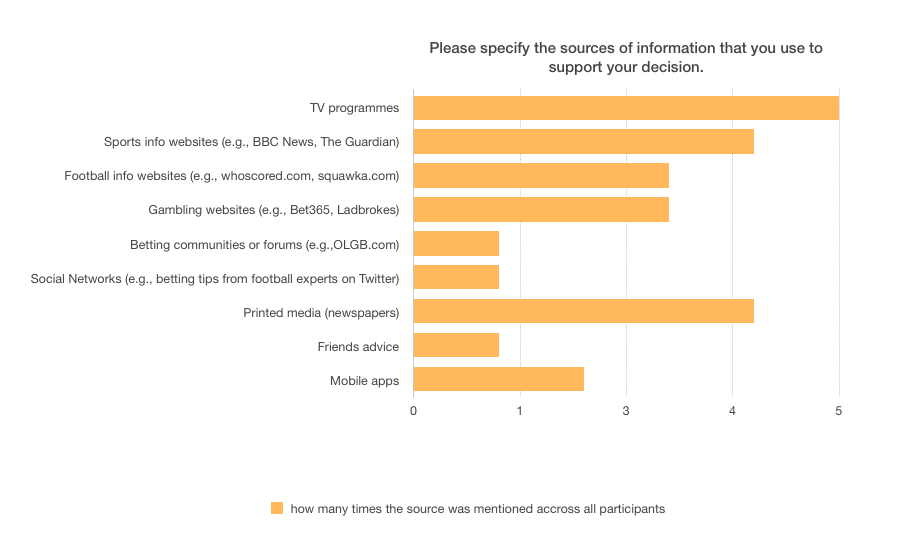
\includegraphics[width=1.0\columnwidth]{req/images/listTheSources.png}
		\caption{A bar chart illustrating the answers of the respondents when asked to specify the sources of information that they use to support a betting decision.}
		\label{fig:using:llistthesources}
	\end{center}
\end{figure}

Charts in figures \ref{fig:using:howmanysources} and \ref{fig:using:llistthesources} demonstrate that punters tend to analyse data from several sources before placing their bets. This proves a need for an application that can reduce the amount of time people spend switching between different type of media to obtain all the information they need. Among the most popular sources were mentioned TV programmes, sports info websites and newspapers.

\begin{figure}[H]
	\begin{center}
		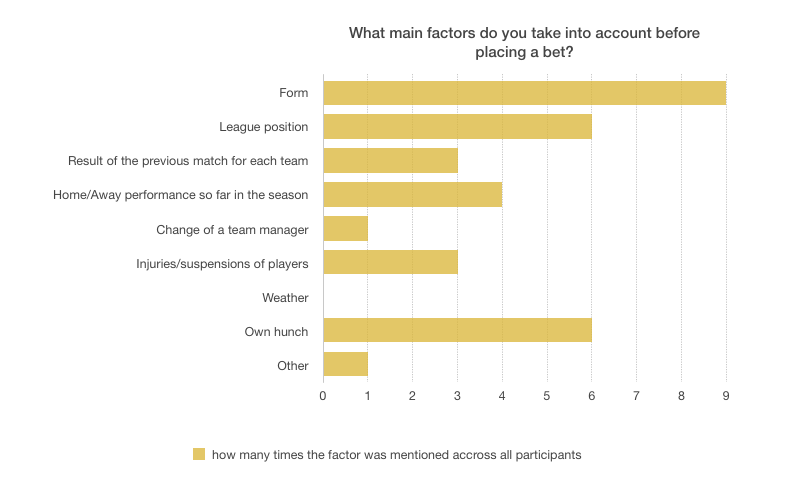
\includegraphics[width=1.0\columnwidth]{req/images/listYourFactors.png}
		\caption{A bar chart illustrating the answers of the respondents when asked to specify the factors they consider before placing a bet.}
		\label{fig:using:listyourfactors}
	\end{center}
\end{figure}

The respondents were asked to list all the factors that they take into consideration before making a betting decision. They were provided with a long list to choose from and asked to specify their own factors if needed. The bar chart in figure \ref{fig:using:listyourfactors} illustrates the answers. Three factors appeared to be clear winners: form, league position and home/away performance. An interesting point is that punters often use intuition in the decision-making process, as 66\% of the respondents mentioned "own hunch" as one of the factors. Incorporating user hunch into the prediction formula will be a clear challenge for me as a developer, however, it looks like the potential application users would like to be able to include it into the calculation.

It was expected that more respondents will mention home/away performance as one of the top influences in making betting decisions. The relatively low interest in this factor can be possibly explained by the fact that the value representing home/away performance cannot be simply found in a standard league table, and a punter needs to make an extra effort to calculate it.

One of the respondents specified a factor that had not been considered in the field "other": "whether or not the odds appear to offer good value". Considering that most survey participants mentioned that they only use one favourite betting provider when placing a bet, this seems to be an interesting point. It looks like the future application will benefit from offering its users odds comparison and possibly a recommendation, such as "odds of the day".

Another interesting fact is that 100% of the respondents answered "no" when asked whether they track their betting performance. The answers prove that monitoring performance seems like a step not worth the added effort for the majority of punters. This observation led me to an idea to consider including a tracking tool into the application because it is definitley a useful thing to have when trying to improve your betting performance and if it does it automatically, i.e. without the added effort, then all the better.

Finally, most of the survey participants answered "yes" when asked whether they would find useful a "web application allowing you to participate in the prediction of a match result by making up you own prediction formula". 

Despite the limited amount of respondents, the answers collected with the questionnaire appeared to be a very valuable input to the phase of the project planning.

\section{Researching Current Solutions}
\label{sec:currentsolutions_req}
Before gathering the project requirements, it is good practice to conduct research on what current websites are already available to football fans with interest in betting. The research can be a source of inspiration and could also help to avoid potential design mistakes. During the analysis, it is important to attempt to understand the main purpose of the analysed websites, as well as the way they present information to the user and communicate with them.

This section is concerned with websites that can be useful for predicting football results. In our context, these are the various online sources of information a football punter would turn to before making a betting decision unless the decision is based solely on intuition. In general, several different types of such websites can be found online, namely:
		
\begin{enumerate}
	\item Sports news websites
	\item Football statistics websites
	\item Bookmakers websites
	\item Communities for sports fans
	\item "Black-box" prediction applications
\end{enumerate}

This section of the report looks at one or two examples of each of the categories presented above, analysing the weak and strong points of the chosen website and discussing usefulness of the whole category from the point of view of a football punter.
	
\subsection{Sports news websites}
\label{subsec:sportsnewswebsites_req}
This category represents football news websites. Into this category fall both general sports websites with a football section and football news websites, such as:
	
\begin{itemize}
	 \item BBC Sport \citep{source:bbcsport}
	 \item The Guardian Sport News \citep{source:guardiansport}
	 \item Sky Sports \citep{source:skysports}
	 \item The Times Sport section \citep{source:thetimes}
	 \item Football365.com \citep{source:football365}
	 \item Goal.com \citep{source:goal}
\end{itemize}

The sports news websites aim to present the news alongside the essential football statistics. The information is usually not as detailed as on the football stats websites, however the very latest football news compensates for this drawback. Each of the \emph{news} websites named above (BBC News, The Guardian, Sky Sports) have a football section that presents the reader with the combination of football news and stats.  One of the most popular football news websites is BBC Sport Football.
	
\subsubsection{BBC Sport Football}
\label{subsubsec:bbcsportfootball_req}
BBC Sport Football is a good quality sports news website. It offers a very neat and simple interface and does not overwhelm the reader with irrelevant graphics. Although, it almost looks too minimalistic, the user can still get all the most important information about football teams and players. The website provides automatically updated live scores across all featured football leagues.

BBC Sport has very impressive news coverage of both major and minor British football leagues, as well as the main european leagues. It can also take pride in high quality writers (journalists) contributing to the website and expert analysis from former players and managers. Being a part of the BBC, it can afford to pay for this extra content, giving it an advantage over most other sports websites. Another benefit is it’s ability to embed video from the television arm of the BBC directly on the website, both highlights of games and interviews with current players and managers, again something that most websites cannot do. 

The main drawback is that the stats are kept to a minimum. This can be a problem for a serious football gambler that wants to analyse the details of the game from all possible angles. However, for the purpose of a fan this level of statistics are sufficient.
	
\begin{figure}[H]
	\begin{center}
		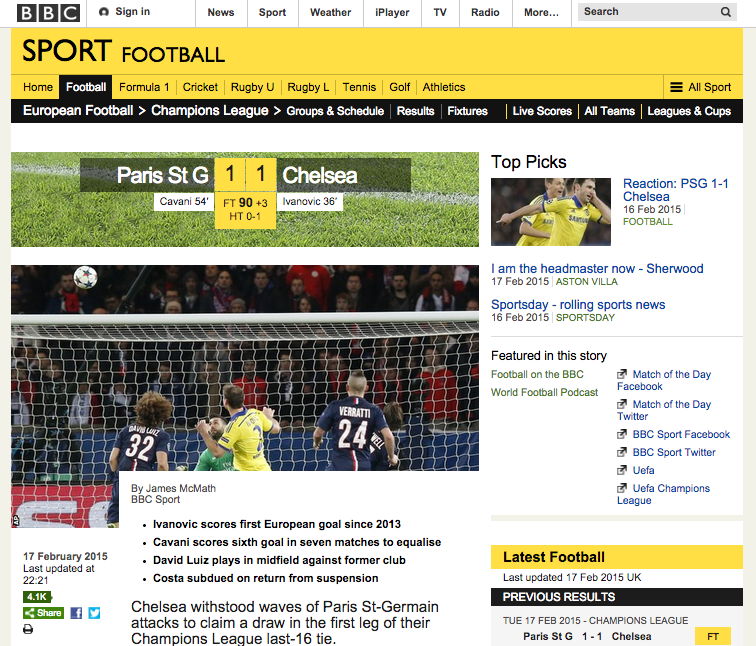
\includegraphics[width=.80\linewidth,natwidth=610,natheight=642]{req/images/bbcsport.png}
		\caption{BBC Sport - Football section} \label{fig:using:bbcsport}
	\end{center}
\end{figure}
		
\subsection{Football statistics websites}
\label{subsec:footballstatswebsites_req}
There is a large selection of football websites dealing in far more detailed statistics and analysis. These are some examples of websites in this category:
			
\begin{itemize}
	\item WhoScored \citep{source:whoscored} 
	\item Squawka  \citep{source:squawka}
	\item Injuries And Suspensions \citep{source:injuriesandsuspensions}
\end{itemize}

\subsubsection{WhoScored}
\label{subsubsec:whoscored_req}
Among all the football stats websites I have analysed, WhoScored is one of the most impressive ones. It has statistics on every possible aspect of a football match, team or player, some of which are less relevant than others (number of throw ins per game is probably not as important as goals scored for example) but it has everything a gambler could want to know before making a bet. It does provide some football news and articles but it is clearly not their main focus and seems a bit amateurish when compared to the bigger news websites.
The website is extremely well designed, and its navigation is intuitive. WhoScored offers statistics and deep analysis on the major European divisions, as well as providing less detailed but still impressive data on over 500 smaller leagues and 15,000 teams. As to the data source, the website is supported by Opta, the largest live sports data company that is used by BBC Sport, Sky Sports and other significant UK sports news providers. 

The way "WhoScored" presents information on particular matches, both upcoming and already played, is detailed while being uncluttered,which makes it both very useful and easy to use. This is definitely an aim of this particular project and I will be using a similar format when designing the website.

\subsubsection{Squawka}
\label{subsubsec:squawka_req}	
Squawka is another website worth looking at.
		
\begin{figure}[H]
	\begin{center}
		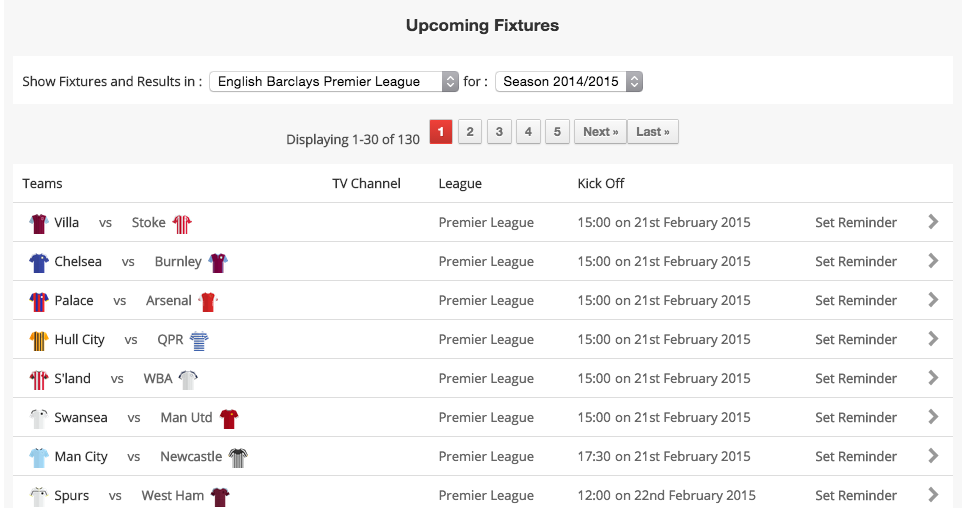
\includegraphics[width=.80\linewidth,natwidth=610,natheight=642]{req/images/squawka.png}
		\caption{Squawka} \label{fig:using:squawka}
	\end{center}
\end{figure}
	
It is an application for football fans that uses real-time data visualisations to show how a game is progressing. The main idea behind it is to show users the live stats as the game is being played and maybe put a bet on “in-play”, for instance it may show that one team is having much more shots on goal than the other so it would make sense to put a bet on them to score the next goal.

From a visual point of view, Squawka has a nicely designed, pleasant interface. However, it is a little bit heavy on the client-side (Javascript), which contributes to sometimes slow performance. Another downside of the website is an extensive amount of adverts that distracts the user form the main content.
	
\subsection{Bookmakers Websites}
\label{subsec:bookmakerswebsites_req}
	
With the arrival of the Internet many existing bookmakers opened up web based operations to complement their existing business. Within short period of time online gambling became very popular with punters all around the world. Most online bookmakers contain high quality sports statistics that aim to support users' betting decisions.

Names like Ladbrokes, Bet365, William Hill are among the most popular bookmakers online, but there are literally hundreds of betting websites now. 
\begin{itemize}
	\item Paddy Power \citep{source:paddypower}
	\item Ladbrokes \citep{source:ladbrokes}
	\item Bet365 \citep{source:bet365}
	\item William Hill \citep{source:williamhill}
\end{itemize}

\subsubsection{Bet365}
\label{susubsec:bet365}

According to the \citet{wiki:bet365}, "Bet 365 Group Limited, is a United Kingdom based gambling company. Bet365 is one of the world’s leading online gambling groups with over 14 million customers in two hundred countries". In my opinion, Bet365 has one of the nicest websites among bookmakers. The website is very well structured, it has intuitive, user-friendly navigation and is easy to use. Bet365 offers a free live streaming service and an impressive coverage of live sports statistics. However, none of the gambling websites I looked at were as intuitive or as thorough with regard to the statistics as Whoscored.com, maybe as they don’t really want their customers to win after all.

\subsection{Communities for sports fans}
\label{subsec:communities_req}
These websites are specialised social networks for sports fans and punters. So far, websites of this type are not particularly popular, maybe because gambling is more of an individual pursuit and gamblers, while liking to be proved right, do not like to share their winning formula with others or alternatively to show that they were wrong.

Many of the features of the websites in this category, such as experts tips, users' comments, forums, can be very useful from a punter's perspective, especially when dealing with a league you are not overly familiar with. I have analysed three websites in this category.
	
\begin{itemize}
	\item OLGB Betting Community - \citep{source:olgb}
	\item Vital Football News and Fans community - \citep{source:vitalfootball}
	\item Punters Lounge - \citep{source:punterslounge}
\end{itemize}

OLGB is a friendly community for punters with many interesting features and tools. It will be analysed in more detail in a separate subsection below. Vital Football is a "network" website. It runs a separate website for every football club from the Premier League and the Football League in England and the Scottish Premier League with each "club site" having their homepage, own editors and a forum. Punters Lounge is a "betting and poker community". Its most interesting feature is a forum for sports gamblers. The website also offers free betting advice tips, live sports streaming and odds comparison.
	
\subsection{OLGB Betting Community}
\label{subsec:olgb_req}
OLGB community market themselves as a website for punters who share their expertise and work together to maximise their betting profit, so it is very relevant to this project. OLGB has a wide variety of features and tools. However, real punters' opinion and tips is the main focus of this website. For example, the user can navigate to an upcoming event page on OLGB website (in the section "free tips") and check how many other users predicted either team to win. Users' choice is usually justified with an comment. For each option OLGB suggests the best odds from one of the most popular bookies. This saves user the trouble of going to a website like OddsChecker\cite{oddschecker} to compare the odds. The comments feature is very interesting and it can be applied as an "optional requirement" for this project.

OLBG also runs a virtual betting game (tipster competition) where users can "bet" virtual money on real betting events. The tipsters in the top 100 of the tables for each sport each month receive a real money prize. Users of the website can also see a leaderboard of the most successful tipsters. The leaderboard contains information on the amount of tips made within certain period of time, LSP (Level Strike Profit), ROI (Return on Investment) for each tipster. The virtual betting feature is very interesting and a leaderboard showing how each user is getting on could be a good way of getting people more involved in my application, probably as an optional feature to avoid losing those users that don’t want to share their wins and losses.

OLGB also has a betting forum, betting blogs section, betting school and much more. The community website has a connection to several popular bookmaker websites. For example, it offers a tool to help users to compare bookmakers websites. It also promotes free bets and various "bookies" promotions.

The website has also several drawbacks. Firstly, the interface is a little outdated and it takes a while to find your way through the complicated and rather confusing navigation. Secondly, the "Help" section only answers some basic questions and can be slightly disorientating for a new user. Again, it’s statistics are not as detailed as the likes of Whoscored and as it is run as a community, the news and information are nowhere near as good as the specific news websites.

\subsection{Black-box prediction applications}
\label{subsec:blackboxapplications_req}
These are betting applications that are marketed as systems that can predict the outcome of a football match using their own unique statistical models and calculations. Known as black-box systems, these applications avoid sharing the exact logic used inside the system with the user. The punter subscribes to a betting system online and simply follows its suggestions for either the estimated outcome of a football match, or on events within a match. For example it may suggest that a lot of goals are likely to be scored in a particular match or even that a lot of corners are likely and therefore the user should bet on that. These are the example apps in this category:

\begin{itemize}
	\item Math Betting \citep{source:mathbetting}
	\item Footbee \citep{source:footbee}
	\item Vitibet \citep{source:vitibet}
	\item Forebet.com - Mathematical Prediction \citep{source:forebet}
\end{itemize}

When paying for the subscription for a black-box betting application, the users assume that they are gaining access to a unique system created by team of experienced football experts. Additionally, there is an expectation that the application has complicated statistical models and calculation analysing a large database of football statistics behind each betting tip. The users also hope that they are paying for a \emph{secret} betting system that is known to and is used by only limited number of other punters. Summing up, a black-box system application sounds like an easy way to sustainable profit. Unfortunately, this does not have to be the case.

According to \citet{art:simplebettingsystem}, the complexity of a betting system does not necessarily correlate with its profitability. The logic behind a successful betting system can be relatively simple and would still work. Secondly, in order to predict a football match result, it may be enough to analyse only relatively recent events (for example last 6 matches, recent players' performance, etc.), without having to perform computations on large set of historic football data. This is due to the fact that over time many various factors can cause change in team performance. Therefore, analysing data from several months ago would not help the punter to make more precise prediction.

\subsection{Conclusion}
After having analysed the above websites, I came to the following conclusion. A well-chosen combination of several websites would definitely be able to provide enough information to make a thoughtful betting decision.

Many punters have their own football betting system (betting strategy) \cite{art:simplebettingsystem}. Although even the best system cannot guarantee success, it can greatly increase the probability of making a profitable bet. Therefore, before making prediction, a thoughtful punter will conduct a little research for each match. The aim of such research would be to collect relevant information about the teams involved in the game. The type of information needed will depend on the \emph{input variables} of the betting system used by each particular punter. The problem is that many football stats websites overwhelm their users with detailed statistics that is irrelevant for prediction purposes. Hence, punters often have to "hand-pick" the important information from several sources for each match.
	
The developed application will attempt to put all the relevant statistics in one place and break the information down into logical modules. In addition, the application will enable users to pick the input variables themselves, and assign them a weight of the user's choice, enabling the user to completely ignore data that they don’t feel is important and focus instead on what matters when deciding on an outcome to bet on. With that comes the ability to improve their system as they go along, they can see what is or isn’t working and hone their system to give them the best possible chance of winning, which is something not provided by the “black box” type applications. 
\section{Requirements Specification}
\label{sec:requirements_req}
\citet{book:radice1998software} define project requirement as follows: "A \emph{requirement} conveys an essential property that the system must or should satisfy." Requirements analysis involves gathering information in order to meet customer needs and defining what the future application is expected to do.
This phase of software engineering is especially important in the industrial environment, when developing an application for a customer. In that case, clarifying the requirements in the early stages of the project would help to ensure that both sides understand and agree on the feature set of the future application.

Although it is not very likely that requirements for this project will change during the development process, defining requirements can be very beneficial. The detailed requirements analysis will aid in the understanding of how different parts of the project are expected to interact with each other, as well as how the application will communicate with its users.

For better transparency, project requirements have been split into functional and non-functional requirements. Functional requirements will be further subdivided into mandatory and optional, depending on the degree of constraints.

Before outlining project requirements, it is good to start with some definitions relevant to the project as a whole.

\subsection{Definitions}
\label{subsec:definitions_req}
\textbf{Application Football League} - in order to reduce unnecessary complexity at this stage of the project, the application will be only supporting one league.

\textbf{Matches Overview} – a list of upcoming and played matches presented on the main page of the website.

\textbf{Dashboard} - an interface available to authorised users. Dashboard is a starting point for users to view, edit and commit saved matches, as well as access other prediction-related content and tools.

\textbf{Prediction Module} – my own term. Each prediction module represents an input system variable in the betting system   
\citep{art:bettingsystemvariableparameters}. The aim of each prediction module is to evaluate and compare in a predefined way blocks of latest football statistics for each of the teams participating in the game (for example, position of each team in the league standings table). The result of this comparison is a module \emph{prediction value} that expresses the probability of either team to win based on one module statistics.

\textbf{Prediction Settings} - a set of weights assigned to prediction values in the betting system in order to forecast the result of the match.

\textbf{System Default Prediction Settings} - the application has a set of "recommended" weights that are used in the prediction calculation by default.
\textbf{User Default Prediction Settings} - each user of the application can override the system default prediction settings and save their own set of weights. From the moment those weights are in the database, they will be applied by default in the prediction calculation for each match saved by the user.

\textbf{Match Specific Prediction Settings} - each user of the application can also save a set of prediction settings applying to only one match.

\textbf{Match result} - "Home Win" in case of the win of the home team, "Away Win" in case of the win of the away team, "Draw" for the draw.

\subsection{Functional Requirements}
\label{sec:functionalrequirements_req}
Functional requirements describe the behaviour of the application in terms of its functionality. These are the "must have" functions of the application addressing the business targets that application must satisfy. Good functional requirements must be complete, coherent and unambiguous.
In order to add structure to the design and development process, the project was logically divided into high level features of the future application. The \emph{mandatory} functional requirements are grouped by the functionality related to these features.

\subsubsection{Authentication and User Profile}
\label{sec:authandprofile_req}
These are the requirements for the basic functionality of the web application, such as account registration, login, logout and account management. The requirements relating to the user profile page will be also listed in this subsection.

\textbf{The application will allow users to register and create a new account with the application.}
\begin{itemize}
 	\item User will be able to register using a standard web form.
 	\item For the registration purposes user will provide a valid email address and a password.
 	\item User will confirm a password in a separate input field.
 	\item On completing the registration form, the application will send the user an email containing a confirmation url.
 	\item On successful confirmation of an email address using the above confirmation url, user will be successfully registered.
 	\item In case of any technical problems with the initial confirmation email, the application will generate a new confirmation url and send it to users on request.
\end{itemize}

\textbf{The application will allow users to sign into their accounts using a standard web form.}
\begin{itemize}
	\item User will provide email address and a password associated with it.
	\item When signing in, user will provide valid credentials, otherwise an application will show a validation error.
\end{itemize}

\textbf{Account management}
\begin{itemize}
	\item The application will enable users to manage their accounts by changing personal information related to it (for example, location, favourite football team) using a web form.
	\item Users will be able to change the email address associated with their account.
	\item Users will be able to change their passwords at any time. 
	\item The application will provide users with a way to recover their lost passwords.
\end{itemize}

\textbf{User profile}
\begin{itemize}
	\item The application will have a special user profile page containing all the essential information about the current user.
	\item Users will also be able to view profile pages of other users of the application.
\end{itemize}

\subsubsection{Matches Overview}
\label{subsubsec:matchesoverview_req}
Below can be found requirements related to the matches overview.
\begin{itemize}
	\item On the main page of the application, user will be presented with a list of upcoming matches for the current season in the league.
   \item User will also be able to view a list of matches already played in the current season and switch between upcoming and played matches using navigation tabs.
  \item Each of the entries in the match list will contain the most basic information about the match, e.g. names of the teams participating in the event, kick-off time and date, full-time score (only for the played matches).
  \item For each of the unplayed matches, user should be able to navigate to the match page and see more details about the match.
 	\item From the main page user will be able to save any unplayed match to the dashboard for a later review.
 	\item For each of the played matches user will be able to navigate to the match page and see more details about the played match.
\end{itemize}

\subsubsection{Prediction}
\label{subsubsec:prediction_req}
In this part of the report, the Prediction feature of the application will be explained and the related requirements will be listed.

The outcome of a football match will be calculated after evaluating several factors that can influence the result. An example of such a factor could be the previous match result, the position in the league, the team’s performance at home or away, a recent change in team management, individual player’s performance, as well as injuries and suspensions of team players. When considered as a part of a betting system, a factor is basically an \emph{input system variable} \cite{art:simplebettingsystem}. As already mentioned above in the "Definitions" \ref{subsec:definitions_req}, each of those input variables will have a "prediction module" representing it in the application and the main outcome of each prediction module will be a "prediction value", percentage that tells the user which team is more likely to win the match.

Finally, the betting system will assign a weight, the value of which will depend on user settings, to each of the prediction values. The weights or prediction settings determine the relative importance of each factor. By applying the weights, the user indicates that some factors are more important to the outcome of this particular game than the others. The final result will be calculated as a weighted average.

As it can be seen from the above explanation, the list of factors that can be considered in the application can be quite long. To simplify the development process, it was decided to limit this list to only three factors. Factors listed below were chosen based on the analysis of the data obtained from the target audience questionnaire \ref{sec:targetaudiencequestionnaire_req}. "League position" and "Form" were two top answers when answering the question

\begin{itemize}
	\item League position of each of the two teams
	\item Form of each of the two teams
	\item Home/Away performance of each of the two teams
\end{itemize}

During the implementation phase these factors will be transformed into prediction modules and integrated into the application. On the top of that, an extra prediction module, "User Hunch" will be created. This is a special module that will allow the users to incorporate their intuition into the prediction calculation and thus influence the result of the prediction. "Own Hunch" was also one of the most common responses among the questionnaire participants.

Below can be found the requirements relating to the prediction feature of the application.

\begin{itemize}
 \item To calculate prediction values for each module, application will use the \emph{system default} settings in absence of either the \emph{user default} prediction settings or the \emph{match specific} settings.
 \item The application will make use of the \emph{user default} prediction settings (explicitly set by the user using a web form) in absence of the \emph{match specific} settings.
 \item The application will apply \emph{match specific} settings if the user has set them for this match.
 \item Match result prediction will be calculated as a weighted average of prediction values using an appropriate set of weights based on the logic outlined above.
\end{itemize}

\subsubsection{Upcoming Match View}
\label{subsubsec:upcomingmatch_req}
For each unplayed match, user should be able to view relevant football statistics, change the match result prediction by adjusting the weights and "commit to bet" the match, once they are satisfied with the final output. Below can be found the requirements illustrating this part of the application functionality.

\textbf{Functionality available for all users.}
\begin{itemize}
	 \item Upcoming match view will contain general information about the match in the view "header", e.g. names of the teams participating in the event, kick-off time and date, the result of the last match for each of the teams.
   \item As well as the match "header", the view will present the user with a list of prediction modules.
   \item Each prediction module will contain the relevant statistic relating to that module.
   \item For each prediction module, it will clearly show which team is more likely to win and what the probability of this outcome is if the match prediction was based solely on this module. In other words, each prediction module will have its \emph{prediction value} clearly indicated.
   \item In case the user has not saved the upcoming match to the dashboard, the view will display only list of prediction modules and associated prediction values. However, it will not be possible to make a match result prediction or commit the match.
  \end{itemize}
 
\textbf{Functionality available for the users who saved the match to the dashboard.}
\begin{itemize}
	\item The user will be able to see what weights are being used for each prediction module.
   \item The application will allow the user to set new match specific prediction weights on this page.
   \item As well as the modules based on the football statistics, the upcoming match view will contain a special module, "user hunch". Its importance was already outlined in the subsection "Prediction" \ref{subsubsec:prediction_req}.
   \item User will be able to commit the match, once satisfied with the result of the prediction.
   \item Once the match is committed, the prediction cannot be changed.
\end{itemize}

\subsubsection{Played Match View}
\label{subsubsec:playedmatch_req}
After the game has been played, the user will be able to navigate to the played match page. The page will contain brief match statistics as well as the summary of the performance of users who placed the bet. This view should be more about the retrospective analysis of the users' betting strategies, i.e. the weights used for modules, rather than the detailed statistics from the actual match, i.e. shots on target, possession, etc. Hopefully, the information presented in this view will allow users to compare their results with the fellow punters and encourage them to analyse their own betting strategy and optimise performance.

These are the requirements relating to the played match view.

\begin{itemize}
	\item Played match view will have a match "header", similar to the header in the upcoming match view.
	\item User will be able to view a brief summary of the pre-match statistics. This information will give the users an idea on how the two participating teams were performing previously to the played match.
	\item Users will be able to see an overview of the website population performance, more specifically performance of users, who committed a bet for this match.
	\item Users will be able to see the visualisation of the website population's choice of prediction weights used for this match, possibly a pie chart.
	\item The view will also have the visualisation, possibly a bar chart, of the website population's choice of the winner for this match (home team, away team or draw).
	\item It should be clear from the view what was the result of the bet for an authenticated user. The view will clearly indicate the user's choice and prediction probability. This part of the view will be only available for users who bet on this match and omitted for the rest of the population.
\end{itemize}

\subsubsection{Dashboard}
\label{subsubsec:dashboard_req}
Dashboard is a key view of the application.

The idea behind the dashboard in this application is similar to online shopping experience: user saves an item to the shopping basket and can later submit a purchase or cancel it. In our case, user browses through the list of matches on the main page of the application and saves matches to the dashboard for a later review. The requirements listed below describe the dashboard functionality in more detail.

\begin{itemize}
   \item User can save a match to the dashboard from the matches overview  \ref{subsubsec:matchesoverview_req}.
   \item User can remove any unplayed or played match from the dashboard.
   \item Dashboard will have a \emph{dashboard menu} holding the links to various tools and views. Suggested entries of this menu are "Upcoming Matches", "Archive", "Prediction Settings".
   \item "Upcoming matches" will be a default view of the Dashboard. It will contain all the saved matches that have not been played yet.
   \item Tab "Archive" will navigate the user to a view containing the saved matches that have already been played.
   \item "Prediction Settings" tab will open a view with a web form, which can be used to save the user default prediction weights.
   \item In the list of saved matches (both upcoming and played), it will be clearly indicated (colour coded) whether a saved match was committed and what the user predicted.
   \item If there are any committed matches in the Archive view, it will be clearly indicated whether the user won or lost a bet.
\end{itemize}

\subsubsection{Notifications}
\label{subsubsec:notifications_req}
The system should be able to notify its users whether they won or lost the bet.
\begin{itemize}
   \item The end of a match is what will trigger new notification messages in the application. Once a game is finished (the full-time score is available), the application will send a notification to the user.
   \item The user will be able to view the list of all notifications.
   \item The user will be able to delete a notification.
   \item The user will be also able possible to delete all notifications from the list.
\end{itemize}

\subsubsection{Leaderboard}
\label{subsubsec:leaderboard_req}
The application will have a Leaderboard, which is a table comparing the current standings of the application users in terms of their betting performance.
\begin{itemize}
   \item The leaderboard table will display players' usernames, their total win and loss points. The table will be sorted in order of win points.    
	 \item Hence, the most successful punters will be on the top of the table.
\end{itemize}

\subsubsection{Optional requirements}
\label{sec:optional_req}
The functional requirements were split into two main groups: mandatory and optional. This is due to the fact that the application was developed over a relatively short period of time and there was not enough time to implement all of the intended functionality. Mandatory requirements represent the "minimum viable product", application developed with the core features that are sufficient to prove the concept of the future product.

On the other hand, the optional requirements illustrate possible improvements that can be made to the application in the future. Additional research will be needed in order to decide which of the features listed below will be the most useful for the target users. The future scenarios of how the application can be extended in the future will be further discussed in the section "Improvements and Future Work" of the chapter "Conclusion".

\begin{itemize}
   \item The application should have more prediction modules. Suggested modules are "Recent change of team management", "Injuries and suspensions of players", "Individual players' performance", "Previous game result", etc.
   \item More football leagues should be supported.
   \item The user should be able to add/remove any prediction module from the Upcoming Match View. This should help keep the focus on only relevant information from the user's point of view.
   \item The application should offer a betting performance tracking tool that will record the details of the past bets and also keep track on whether the punter is profitable in the long run.
   \item The application should offer its users odds comparison functionality. It is a known fact that the odds for the same event may vary considerably between different bookmakers. The application should compare the odds across the most popular bookmakers and suggest the best option with regards to the user's prediction (home win, away win or draw). Clicking on the suggested odds should take the user to the bookmaker's website or open a bet slip.
   \item The application should get some features of a sports fans community. Users should be able to leave comments on each match explaining the prediction they made and also follow each other. Followers should see the comments from the followed users in their news feed. The news feed should be accessible from the dashboard. 
    \item The application should implement "Sign In with Facebook" functionality allowing its users to login with a single click.
\end{itemize}

\subsection{Non-functional Requirements}
\label{sec:nonfunctional_req}
Non-functional requirements specify how the system is going to perform.

\begin{itemize}
	\item \textbf{Usability} - The application interface should be easy to understand and learn for a new user. The navigation of the website should be highly intuitive.
	\item \textbf{Responsiveness} - The application should be fully responsive. The websites will be tested for a variety of screen resolutions and the minimum screen resolution will be 640x960 (DVGA - iPhone).
	\item \textbf{Performance} - Optimising performance will be crucial for the application, as there is a direct correlation between the application response time and the user experience.  Performance problems will be detected and eliminated as soon as they appear.
	\item \textbf{Cross-browser support} - The application will be supported on a minimum set of web browsers, such as Chrome, Internet Explorer 9+, Safari, Firefox.
	\item \textbf{Maintainability} - The focus should be on delivering clear and maintainable code. The code needs to be easily understandable by other developers. For this purpose the best practices of software development and the used languages will be utilised throughout the implementation phase of the project.
	\item \textbf{Extensibility} – The system will be developed with a large-scale application in mind. It should be easy to apply ongoing changes to the project.
\end{itemize}

\section{Overall Architecture}
\label{overallarchitecture_req}
The high level components of this system are quite simple.

Design of an application a a whole, overall design (just boxes and lines)
Architectural diagram (overview) (aosabook.org/en/moodle.html -example), quite high level


\section{Choice of Third Party API}
\label{sec:thirdpartyapi_req}
	
After analysing the functional requirements, it became apparent that this type of application will need the latest football data in order to operate correctly. The easiest way to load data into the application would be to integrate the application with a third party API. The process of finding an appropriate API for the project will be described in this section.
	
After brief research, one thing became apparent. Live football data is a very desirable product and therefore it is not easy to find free of charge live football data API. The key problem is that the data has to be very recent. Real-time data in particular is very expensive, because of its use by the gambling industry for betting on various markets as the games are going on. It is actually much easier to find free historical football data. 
	
This is a list of API providers that have been researched and evaluated.
	
\begin{itemize}
	\item Optasports.com \citep{source:opta}.\par
Opta is the industry leader. It provides a wide range of XML feeds covering many sports. The feeds include fixtures and results, live scores, live player stats and many more. Data provided by Opta is very reliable and is used by top-notch clients, such as BBC Sports, BT Sport, Sky Sports, as well as many betting providers and newspapers.		
	\item Openfooty \citep{source:openfooty}.\par
	Openfooty is an interesting project with very detailed API documentation. However, a quick look at the developer forums shows a stale community and many questions about why no one seems to actually be able to get a developer key. Unfortunately, I also did not manage to obtain a key for this API.			
	\item Football API \citep{source:footballapi} .\par
This is a paid API service. The API restricts by IP addresses and limit calls based on the package. On the bright side, it offers the English Premier League endpoints for free (demo use). The API includes endpoints for competitions, teams, standings, live scores, fixtures and commentaries.	
	\item XML Soccer \citep{source:xmlsoccer}. \par
	Another paid API service that offers full access to the Scottish Premier League data for free.
		
\end{itemize}
	
Football API was chosen to be integrated with the application. As already mentioned in the "Definitions" \ref{subsec:definitions_req}, it was decided to support only one league for the time being. Football API offers its users free access to the English Premier League, which seems to be a great choice for our application, as this league's worldwide popularity will hopefully make it easier to find other league-related data and information that might be needed during the development process.

\section{Project Plan}
\label{projectplan_req}
The project progress timetable is presented in the Gantt diagram below. Two main milestones were set for this project: firstly, to develop the first prototype of the application and secondly, to complete the second prototype by the end of April, 2015 (this includes all the testing and bug fixes).

The first prototype will have implemented most of the high level features of the application as introduced in the section "Requirements" \ref{sec:requirements_req}. The second prototype is a more refined version of the application; it will implement all mandatory requirements listed above and have the visual side of the website polished up.



